% ------------ HEADER ------------ %

% DOCUMENT: ENERGY 295 Final Project Report Equations
% AUTHOR: Miles Smith
% DUE DATE: 7 December 2021


% ------------ PREAMBLE  ------------ %


\documentclass[12pt]{article}
\usepackage{times}
\usepackage[margin=1in]{geometry}
\usepackage{amsmath,amsthm,amssymb}
\usepackage{graphicx}
\usepackage{multirow}
\usepackage{setspace}
\usepackage{subcaption}
\usepackage{caption}
\onehalfspacing


% ------------ DOCUMENT ------------ %

\begin{document}

\title{ENERGY 295 Lab Report Equations}
\date{\today}
\author{Jessica, Tom, Miles}

\maketitle
\tableofcontents
\clearpage

\section{State Equations}
\par
Beginning with a second-order equivalent circuit model for a Li-ion battery,

\begin{figure}[h]
\centering
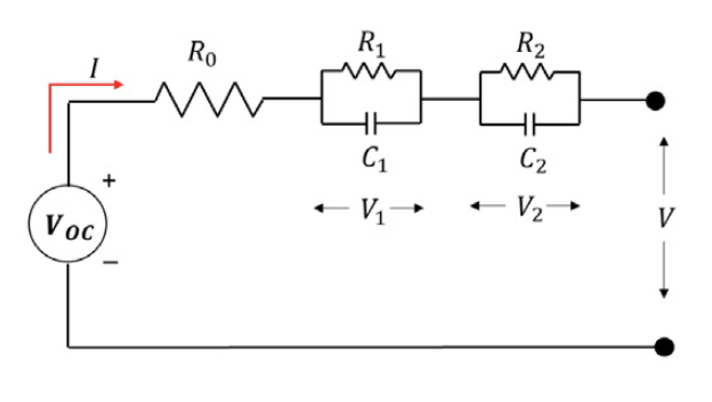
\includegraphics{ECM.png}
\end{figure}

The cell voltage, V, is mathematically defined as,

\begin{equation}
\centering
V(t) = V_{OC}(SOC) - V_1(t) - V_2(t) - R_0(SOC)\;I(t)
\end{equation}


and applying a general state-space representation to the system, such that

\begin{equation}
\centering
\dot{x}(t) = Ax(t) + Bu(t)
\end{equation}

\begin{equation}
\centering
y(t) =  Cx(t) + Du(t)
\end{equation}

In this model, we initially do not consider $R_0$ as a state variable that responds to system noise.  Rather it is considered to be a pure function of SOC, so our state vectors are considered to be 

\begin{equation}
\centering 
x(t) =
\begin{bmatrix}
SOC \\ V_1 \\ V_2 
\end{bmatrix}
\end{equation}

thus, our equations of state are 

\begin{equation}
\centering
\dot{x}(t) = \;
\begin{bmatrix}
\dot{SOC} (t) \\
\dot{V_1} (t) \\
\dot{V_2} (t) \\
\end{bmatrix} 
= \;
\begin{bmatrix}
\frac{-I(t)}{Q_n} \\
\frac{-1}{R_1(SOC(t))C_1(SOC(t))}V_1(t) + \frac{1}{C_1(SOC(t))}I(t) \\
\frac{-1}{R_2(SOC(t))C_2(SOC(t))}V_2(t) + \frac{1}{C_2(SOC(t))}I(t) 
\end{bmatrix}
\end{equation}

Thus our coefficient matrices, A, B, C, and D, can be defined as 

\begin{equation}
\centering
\begin{matrix}
A = \;
\begin{bmatrix}
0 & 0 & 0  \\
0 & \frac{-1}{R_1(SOC(t))C_1(SOC(t))} & 0  \\
0 & 0 & \frac{-1}{R_2(SOC(t))C_2(SOC(t))}  \\
0 & 0 & 0 \\
\end{bmatrix} 

& 

B = 
\begin{bmatrix}
\frac{-1}{Q_n} \\
\frac{1}{C_1} \\
\frac{1}{C_2} \\
\end{bmatrix}

\\

C = \begin{bmatrix}

(\frac{\partial{V_OC}}{\partial{SOC}} - \frac{\partial{R_0}}{\partial{SOC}}I(t)) & -1 & -1

\end{bmatrix}^*

&

D = \begin{bmatrix}
\bold{0}
\end{bmatrix}
\end{matrix}
\end{equation}

\par
Assuming there is some sort of process noise in the state vector $\dot{x}$ and observation noise at time instance k that are both Gaussian in their distribution with a mean of 0, the discrete time linear system can be described as 

\begin{equation}
\centering
\begin{matrix}
x(k) = Ax(k-1) + Bu(k-1) + w &&
y(k) = Cx(k) + \nu
\end{matrix}
\end{equation} 

The covariance of $w$ is defined as $Q$ and the covariance of $\nu$ is defined as R.  By applying the Jacobian to linearize the coefficient matrices, we get the matrices in their discrete form, such that

\begin{equation}
\centering
\begin{matrix}
A_k = \:
\begin{bmatrix}
0 & 0 & 0 \\
\frac{C_1\frac{\partial{R_2}}{\partial{SOC}} + R_1\frac{\partial{C_1}}{\partial{SOC}}}{(R_1C_1)^2} & \frac{-1}{R_1C_1} & 0 \\
\frac{C_2\frac{\partial{R_2}}{\partial{SOC}} + R_2\frac{\partial{C_2}}{\partial{SOC}}}{(R_2C_2)^2} & 0 & \frac{-1}{R_1C_1}\\
\end{bmatrix}
& B_k = 
\begin{bmatrix}
\frac{-1}{Q_n} \\
\frac{1}{C_1} \\
\frac{1}{C_2} 
\end{bmatrix} \\ \\
C_k = 
\begin{bmatrix}
(\frac{\partial{V_OC}}{\partial{SOC}} - \frac{\partial{R_0}}{\partial{SOC}}I(t)) & -1 & -1
\end{bmatrix} &

D_k = 
\begin{bmatrix}
\bf{0}
\end{bmatrix}
\end{matrix}
\end{equation}

the system can be now be considered using linear modeling techniques. 

\subsection{Considering R$_0$ as a state variable}

\par
Expanding on the previous system, R$_0$ can be considered as a state variable that adapts based on the observation and process noise of the system. The new state vector of the system now is considered to be 

\begin{equation}
\centering x(t) =
\begin{bmatrix}
SOC \\ V_1 \\ V_2 \\ R_0
\end{bmatrix}
\end{equation}

with state variables that are defined as 

\begin{equation}
\centering
\dot{x}(t) = \;
\begin{bmatrix}
\dot{SOC} (t) \\
\dot{V_1} (t) \\
\dot{V_2} (t) \\
\dot{R_0} (SOC(t)) \\
\end{bmatrix} 
= \;
\begin{bmatrix}
\frac{-I(t)}{Q_n} \\
\frac{-1}{R_1(SOC(t))C_1(SOC(t))}V_1(t) + \frac{1}{C_1(SOC(t))}I(t) \\
\frac{-1}{R_2(SOC(t))C_2(SOC(t))}V_2(t) + \frac{1}{C_2(SOC(t))}I(t) \\
0
\end{bmatrix}
\end{equation}

The non-linear coefficients matrices are defined as, 

\begin{equation}
\centering
\begin{matrix}
A = \;
\begin{bmatrix}
0 & 0 & 0 & 0 \\
0 & \frac{-1}{R_1(SOC(t))C_1(SOC(t))} & 0 & 0 \\
0 & 0 & \frac{-1}{R_2(SOC(t))C_2(SOC(t))} & 0 \\
0 & 0 & 0 & 0 \\
\end{bmatrix} 
&
B = 
\begin{bmatrix}
\frac{-1}{Q_n} \\
\frac{1}{C_1} \\
\frac{1}{C_2} \\
0
\end{bmatrix} 

\\ \\

C =
\begin{bmatrix}
(\frac{\partial{V_OC}}{\partial{SOC}} - \frac{\partial{R_0}}{\partial{SOC}}I(t)) & -1 & -1 & -I(t) 
\end{bmatrix}^* &

D = 
\begin{bmatrix}
\bf{0}
\end{bmatrix}

\end{matrix}
\end{equation}

By applying the Jacobian to linearize the system dynamics, the discretized coefficient matrices are developed for each time-instance k

\begin{equation}
\centering
\begin{matrix}
A_k = \:
\begin{bmatrix}
0 & 0 & 0 & 0 \\
\frac{C_1\frac{\partial{R_2}}{\partial{SOC}} + R_1\frac{\partial{C_1}}{\partial{SOC}}}{(R_1C_1)^2} & \frac{-1}{R_1C_1} & 0 & 0 \\
\frac{C_2\frac{\partial{R_2}}{\partial{SOC}} + R_2\frac{\partial{C_2}}{\partial{SOC}}}{(R_2C_2)^2} & 0 & \frac{-1}{R_1C_1} & 0 \\
0 & 0 & 0 & 0 & \\
\end{bmatrix}
& B_k = 
\begin{bmatrix}
\frac{-1}{Q_n} \\
\frac{1}{C_1} \\
\frac{1}{C_2} \\
0 \\
\end{bmatrix} 

\\ \\

C_k = 
\begin{bmatrix}
(\frac{\partial{V_OC}}{\partial{SOC}} - \frac{\partial{R_0}}{\partial{SOC}}I(t)) & -1 & -1 & -I(t) 
\end{bmatrix} &

D_k = 
\begin{bmatrix}
\bf{0}
\end{bmatrix}
\end{matrix}
\end{equation}

\section{Extended Kalman Filter}

\par
To estimate the state variables, $\hat{x}_0$ and $\hat{P}_0$ need to be initialized. These were initialized as 

\begin{equation}
\centering
\begin{matrix}
\hat{x}_0 = 
	\begin{bmatrix}
	SOC_0 & 0 & 0 & 0 \\
	0 & V_{1,0} & 0 & 0 \\
	0 & 0 & V_{2,0} & 0 \\
	0 & 0 & 0 & R_{0,0} \\
	\end{bmatrix} & 

\hat{P}_0 = 
	\begin{bmatrix}
	0.1 & 0 & 0 & 0 \\
	0 & 0.001 & 0 & 0 \\
	0 & 0 & 0.001 & 0 \\
	0 & 0 & 0 & 0.001 \\
	\end{bmatrix} 

\end{matrix}
\end{equation}

The process noise, $Q$ and its dependent measurement noise $R$ are also initialized. The measurement noise, R, is set as 

\begin{equation}
\centering
R = 1 \times 10^{-4}
\end{equation}

and the process noise matrix, $Q$, is set as 

\begin{equation}
\centering
Q = 
	\begin{bmatrix}
	100R & 0 & 0 & 0 \\
	0 & 0.1R & 0 & 0 \\
	0 & 0 & 0.01R & 0 \\
	0 & 0 & 0 & 0.1R \\
	\end{bmatrix}
\end{equation}

Using the prior estimation (k-1) of the states the EKF will estimate the state variables and process noise at discrete time instance, k. The initial prediction of the states and process noise covariance at time instance k are described as,

\begin{equation}
\centering
\begin{matrix}

\hat{x}_{k|k-1} = A_k \hat{x}_{k-1|k-1} + B_k u_{k-1} \\ \\

P_{k|k-1} = A_k P_{k-1|k-1} A_k^T + Q

\end{matrix}
\end{equation}

To correct the system difference between the prediction step and the true value, a gain (Kalman Gain, $L$ is estimated for a time instance k, such that 

\begin{equation}
\centering
L_{k} = \frac{P_{k|k-1} C_{k-1}}{C_k P_{k|k-1} C_{k-1}^T + R}
\end{equation}

Thus, the corrected estimations of $\hat{x}_k$, $\hat{y}_k$, $P_{k}$ are described as 

\begin{equation}
\centering
\begin{matrix}
	\hat{x}_k = \hat{x}_{k|k-1} + L_{k}(y_{k} - \hat{y}_{k|k-1}) \\ \\
	\hat{y}_k = C_k\hat{x}_k \\ \\
	P_{k} = (\bold{I} - L_k C_{k-1})P_{k|k-1}
\end{matrix}
\end{equation}

\subsection{Adaptive Extended Kalman Filter}

\par
Modifying the system to an adaptive EKF expands upon a traditional EKF by adding an innovation covariance matrix at each time instance, $\hat{D}_k$, and an adaptive noise covariance matrix, $\hat{Q}_k$, such that,

\begin{equation}
\centering
\begin{matrix}
	\hat{D}_k = \frac{1}{N}\sum\limits_{i=i_0}^{k} d_i d_i^T \\ \\ 
	\hat{Q}_k = L_k \hat{D}_k L_k^T
\end{matrix}
\end{equation}

where,

\begin{equation}
d_{i,k}= y_k - \hat{y}_{k|k-1}
\end{equation}

\begin{equation}
i_0 = k - N + 1
\end{equation}

which gives a noise covariance matrix, $Q$, that adapts for each time step based on the previous N time instances. 

\section{System Performance}

\begin{figure}[h]
\centering
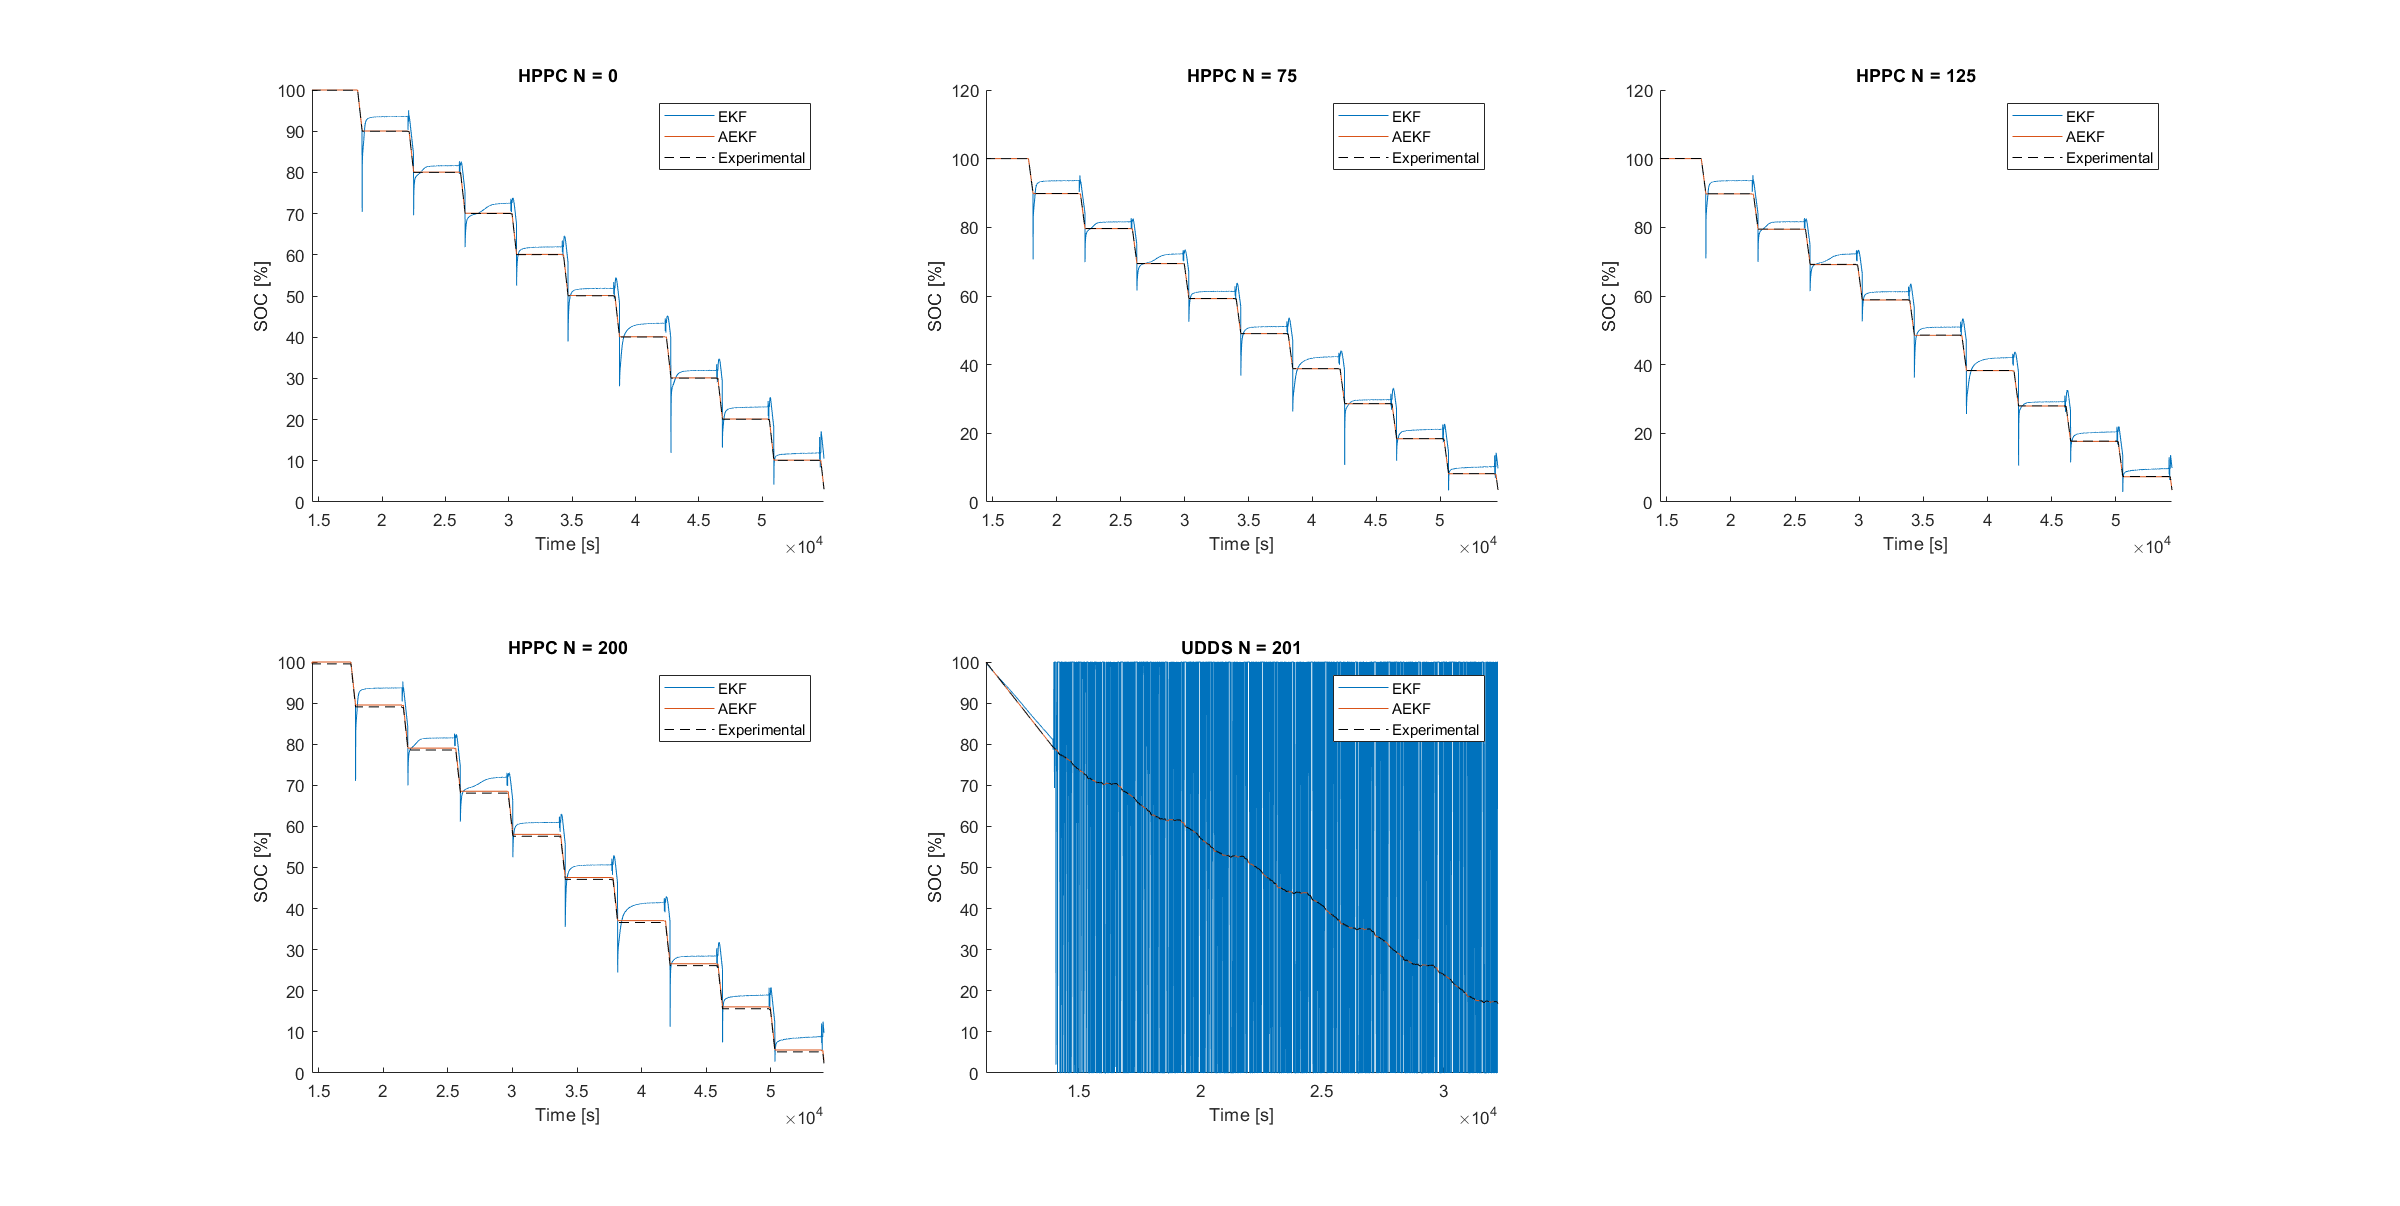
\includegraphics[width=\linewidth]{SOC plots.png}
\end{figure}

\begin{figure}[h]
\centering
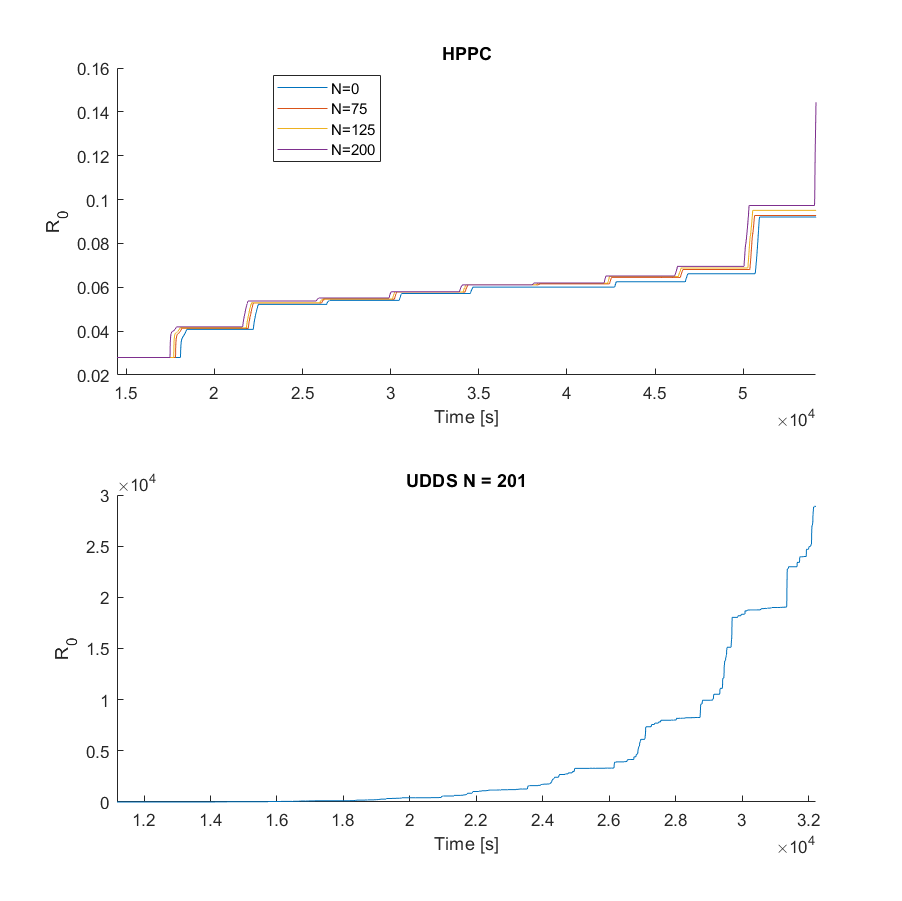
\includegraphics[width=\linewidth]{R0 plots.png}
\end{figure}






















\end{document}

% ------------ END OF DOCUMENT ------------ %
